\documentclass[journal]{../IEEEtran}

\usepackage{graphicx}
\usepackage{fancyhdr}
\usepackage{epsfig} % for postscript graphics files
\usepackage{graphics} % for pdf, bitmapped graphics files

\graphicspath{{Figures/}}

\pagestyle{fancy}
\lhead{CPE 470/670}
\rhead{\thepage}
\chead{Team 6: Lab 7 Report}
\lfoot{}
\rfoot{}
\cfoot{}

\begin{document}

\begin{titlepage}
    \vspace*{\fill}
    \begin{center}
      {\LARGE \bf Lab 7: Soccer Robot}

      {Team 6: Alexander  C. Woods and Taylor Mansfield}

      November 5, 2014
    \end{center}
    \vspace*{\fill}
  \end{titlepage}


\section{Hardware and Software Design}\label{S.design}
\IEEEPARstart{P}{laying} soccer with a robot is a fun and interesting challenge. The robot must be able to sense the location of the ball, determine whether or not it should be attacking or defending, and act accordingly. The field on which the robots played is shown in Fig.~\ref{F.field}. The field consists of a goal on each end, which span the entire width. The goals are marked by black zones and the ball must completely enter the zone in order to be considered a point.

%\begin{figure}[ht]
%\centering
%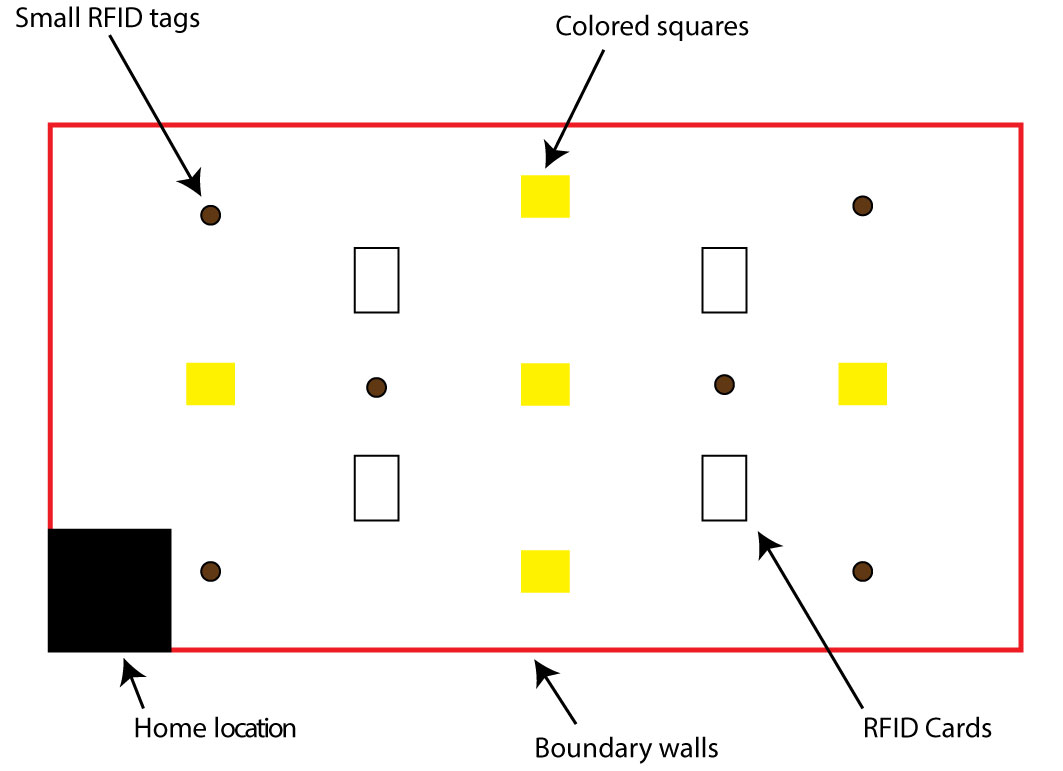
\includegraphics[width=1\columnwidth]{field.jpg}\\
%\caption{The field on which the robots play soccer has a goal on each end which spans the width of .}
%\label{F.ramp}
%\end{figure}

The sensors used for this challenge are quite simple. An IR sensor is used to detect the location of the ball according to the map shown in Fig.~\ref{F.ir_map.eps}. The only other sensor used in this challenge is a compass sensor which is used to determine the heading of the 

An ultrasonic sensor is equipped which lets the robot sense and avoid wall while it is looking for balls. The ultrasonic sensor is strategically located on the left side of the robot as shown in Fig.~\ref{F.us_sensor} so that it can sense walls, but will not be fooled by a ball. This is because the robot keeps the wall on its left side naturally. If the robot were to use a right sided wall following technique instead the ultrasonic sensor would be located on the other side of the robot.

\section{Problems Encountered}\label{S.problems}

To begin, we needed a software design to detect and move toward the IR ball. Due to the lack of granularity with the provided sensor and the degree of control we had over the motors, we had some trouble coupling the sensor input to the power of the motors in an effective and meaningful way.

Regarding the form factor of the robot, it was constantly up for debate and restructuring. We had to meet the demands of effectiveness, stability, simplicity, and minimum weight.

We had an issue with backing up from a wall, should we ever run into it, in which the regulation of the power to the wheels prevented them from stopping, which caused the odometry watch to not trigger the backup procedure.

We also had an issue where the robot would behave in a very unexpected way and instead of kicking the ball, would retrieve it and project it toward its own goal.

\section{Solutions}\label{S.solutions}

To drive the motors, we initially tried PID control with input from the IR sensor dir value. This worked mildly well, but had limitations when going up to the ball. We found that there was a serpentining effect when the robot would get close to the ball. In some cases the robot would get really close to the ball and stop short of actually touching it. 

After many iterations, additions, subtractions, and adjustments, we finally came up with a design that would follow our proposed gameplay strategy effectively. With a simple wedge tapering to forward sections, our robot could kick the ball in a random direction downfield (sometimes away from other players), hold the ball against the wall, and with some implementations of software, handle the ball very nicely.

We also attempted to couple the speed of the motors to the observed distance away from the ball, but that implementation had similar problems, especially when trying to overcome an obstacle such as a wall where the robot could not provide enough torque with this algorithm to move past the wall if the ball was close enough to the robot.

We even tried a more simple method of porportional control with different functions applying to different ranges in the sensor direction imput, but while that seemed effective, it drastically lowered the speed of the robot to the point where it was uncompetitive with other robots.

Instead, we went with a case switch statement where we manually set a static value power to the motors, mirrored over the IR sensor's range of directional values and increased in power and decreased in power ratio as the sensor direction approached the forward range. This seemed to have the most effective results, although it was also not perfect (see below).

\section{Unsolved Problems}\label{S.unsolved}

Unfortuantely, we never did solve the issue of the unexpected ball retrieval. In some instances, the ball would be kicked into the opponents goal as normal, whereas in other cases the robot would immediately retieve the ball from the center of the field. This behavior appears to be essentially random, and more fine tuning of the motor speed tied to the sensor input might have fixed the issue. regulating the speed of the motor may have also helped, but that would have caused more issues with recovering from sticking to walls.

\end{document}
